\chapter{支点が水平方向に可動な単振子}

\section{モデルの定式化}

%\begin{comment}
\begin{figure}[htbp]
  \begin{minipage}[b]{0.45\linewidth}
    \centering
    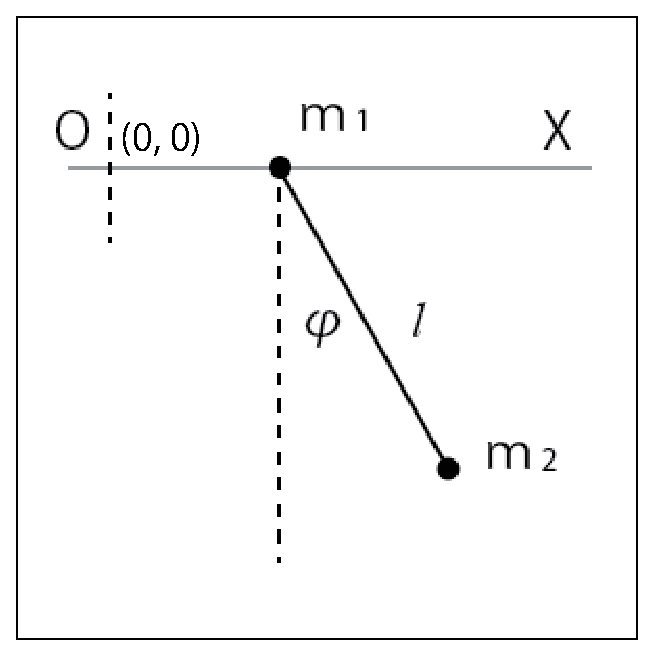
\includegraphics[keepaspectratio, scale=0.6]{movableh.eps}
    \caption{質量$m_1$の支点に質量$m_2$の単振子}
  \end{minipage}
  %\begin{minipage}[b]{0.45\linewidth}
    %\centering
    %\includegraphics[keepaspectratio, scale=0.35]{p13-2.eps}
    %\caption{p13-2}
  %\end{minipage}
\end{figure}
%\end{comment}

質量$m_2$の単振子.その支点である質量$m_1$の質点が水平方向に運動できる.

水平に運動している質点$m_1$の運動エネルギーは、

\[T_1 = \displaystyle\frac{m_1}{2}\dot{x}^2\]

質点$m_2$のデカルト座標$(x_2,y_2)$は、

\begin{align*}
   x_2 &= x + l\sin\varphi \quad,\quad y_2 = -l\cos\varphi\\
   \dot{x}_2 &= \dot{x} + l\dot{\varphi}\cos\varphi \quad,\quad \dot{y}_2 = l\dot{\varphi}\sin\varphi\\
   \dot{x}_2^2 &= \dot{x}^2 + 2\dot{x}l\dot{\varphi}\cos\varphi + l^2\dot{\varphi}^2\cos^2\varphi \quad,\quad \dot{y}_2^2 = l^2\dot{\varphi}^2\sin^2\varphi
\end{align*}

質点$m_2$の運動エネルギーは、$\sin^2\alpha+\cos^2\alpha=1$を思い出して、

\[T_2 = \displaystyle\frac{m_2}{2}\left(\dot{x}_2^2+\dot{y}_2^2\right) = \displaystyle\frac{m_2}{2}\left(\dot{x}^2 + 2l\dot{x}\dot{\varphi}\cos\varphi+l^2\dot{\varphi}^2\right)\]

一方、ポテンシャル・エネルギー$U$は、

\[U = -m_2gl\cos\varphi\]

従って、Lagrangian$L=T_1+T_2-U$は、

\[L=\displaystyle\frac{m_1+m_2}{2}\dot{x}^2+\frac{m_2}{2}\left(l^2\dot{\varphi}^2+2l\dot{x}\dot{\varphi}\cos\varphi\right)+m_2gl\cos\varphi\]

Euler-Lagrange eq.は,次の計算をして、

\begin{align*}
   \frac{\partial L}{\partial\dot{\varphi}}&=m_2l^2\dot{\varphi} + m_2l\dot{x}\cos\varphi \qquad,\quad \frac{\partial L}{\partial \varphi} = -m_2l\dot{x}\dot{\varphi}\sin\varphi - m_2gl\sin\varphi\\\\
   \frac{\partial L}{\partial \dot{x}} &= (m_1+m_2)\dot{x} + m_2l\dot{\varphi}\cos\varphi \qquad,\quad \frac{\partial L}{\partial x}=0
\end{align*}

従って,

\begin{align*}
   &m_2l^2\ddot{\varphi}-m_2l\dot{x}\sin\varphi = -m_2l\dot{x}\dot{\varphi}\sin\varphi - m_2gl\sin\varphi\\\\
   &\therefore \qquad \ddot{\varphi} = \frac{\sin\varphi}{l}\dot{x}+\frac{-\sin\varphi}{l}\dot{x}\dot{\varphi}+\frac{-g}{l}\sin\varphi
\end{align*}

もう一方の式は,

\begin{align*}
   &(m_1+m_2)\ddot{x}+m_2l\dot{\varphi}\cos\varphi=0\\\\
   &\therefore \qquad \ddot{x}=\displaystyle\frac{-m_2l\dot{\varphi}\cos\varphi}{m_1+m_2}
\end{align*}

\section{Pythonによる模擬実験}

これらを連立の一階微分方程式に直すと

\begin{align*}
   \displaystyle\frac{\mathrm{d}\varphi}{\mathrm{d}t}&=\dot{\varphi}\\\\
   \displaystyle\frac{\mathrm{d}x}{\mathrm{d}t}&=\dot{x}\\\\
   \displaystyle\frac{\mathrm{d}\dot{\varphi}}{\mathrm{d}t}&=\displaystyle\frac{\sin\varphi}{l}\dot{x}+\frac{-\sin\varphi}{l}\dot{x}\dot{\varphi}+\frac{-g}{l}\sin\varphi\\\\
   \displaystyle\frac{\mathrm{d}\dot{x}}{\mathrm{d}t}&=\displaystyle\frac{-m_2l\dot{\varphi}\cos\varphi}{m_1+m_2}
\end{align*}

2つの質点の座標$(x,y),(x_2,y_2)$については、座標$x$はラグランジアンに陽に含まれていないことから循環的な座標である.(ランダウ「力学」p.37)循環座標が存在する場合の運動方程式の積分は簡単化できて、$x$を含まない$L$を$x$で微分しても、その結果は定数(ゼロ)になる.

\[\displaystyle\frac{\mathrm{d}}{\mathrm{d}t}\frac{\partial L}{\partial \dot{x}}=\frac{\partial L}{\partial x}=0\]

時間微分$\displaystyle\frac{d}{dt}$の結果がゼロなので、$\displaystyle\frac{\partial L}{\partial\dot{x}}$は定数.

\[\displaystyle\frac{\partial L}{\partial \dot{x}}=(m_1+m_2)\dot{x}+m_2l\dot{\varphi}\cos\varphi=const.\]

これは系の運動量が保存することを表している.この式の積分は、
$(m_1+m_2)x + m_2l\sin\varphi = const.$,$const=0$に対して$x$が次の通り求まる.(ランダウ「力学」p.42 問3)

\begin{align*}
   x&=\frac{-m_2l\sin\varphi}{m_1+m_2}\\
   y&=0\\
   x_2&=x+l\sin\varphi\\
   y_2&=-y-l\cos\varphi
\end{align*}

支点の質量$m_1$を大きくして模擬実験を試すと、固定支点の状態に近づいてくる.($m_1\rightarrow\infty$で$x\rightarrow 0$,これは通常の単振子だ.)

\lstset{escapechar=@,style=custompy}
\lstinputlisting[caption=支点が水平方向に可動な単振子,label=pythonProgram3]{movableh.py}
